\documentclass{article}

\usepackage[utf8]{inputenc}
\usepackage[T1]{fontenc}
\usepackage[norsk,english]{babel}   %Norsk først så engelsk, så engelsk blir prioritert
\usepackage{graphicx}
\usepackage{amsmath}        %For å kunne skrive matte
\usepackage{listings}       %For å kunne skrive inn kode med fin formatering
\usepackage{multicol}       %Importerer pakken for multikolonner til teksten
\usepackage[margin=2.54cm]{geometry}    %Definerer hva bredden til teksten er
\usepackage{wrapfig}    %Importerer pakken for å ha bildene i teksten
\usepackage[font = small]{caption}

%Definerer hyperlinker og dens farger
\usepackage{hyperref}
\hypersetup{
    colorlinks,
    citecolor=blue,
    filecolor=black,
    linkcolor=blue,
    urlcolor=blue
}


%-----------------------------------

%Definerer farger til kodeeksemplene i PDF-en
\usepackage{color}

\definecolor{codegreen}{rgb}{0,0.6,0}
\definecolor{codegray}{rgb}{0.5,0.5,0.5}
\definecolor{codepurple}{rgb}{0.58,0,0.82}
\definecolor{backcolour}{rgb}{0.95,0.95,0.92}

\lstdefinestyle{mystyle}{
    backgroundcolor=\color{backcolour},
    commentstyle=\color{codegreen},
    keywordstyle=\color{magenta},
    numberstyle=\tiny\color{codegray},
    stringstyle=\color{codepurple},
    basicstyle=\footnotesize,
    breakatwhitespace=false,
    breaklines=true,
    captionpos=b,
    keepspaces=true,
    numbers=left,
    numbersep=5pt,
    showspaces=false,
    showstringspaces=false,
    showtabs=false,
    tabsize=2
}

\lstset{style=mystyle}

%------------------------------------

\setlength{\parindent}{0pt} %Ingen indent automatisk for nye linjer
%\setlength{\columnsep}{2mm} %Column separation - til multicolumn

%\setlength{\arrayrulewidth}{1mm}   %Hvilken tykkelse tabellene skal ha
\setlength{\tabcolsep}{3mm}     %Lengden mellom hver kolonne
\renewcommand{\arraystretch}{1.5}   %Hvor stor avstand det skal være mellom radene

\iffalse    %midlertidig endre bredden på teksten
If you want to change this temporarily, you can write:
\savegeometry{mydefaultgeometry}
\newgeometry{margin=3in}
And then later you can call:
\loadgeometry{mydefaultgeometry}
\fi

%for å fjerne overskriften "refrences" som kommer automatisk når man bruker bibtex
\usepackage{etoolbox}
\patchcmd{\thebibliography}{\section*{\refname}}{}{}{}

% To avoid LaTeX re-positioning tables and images
\usepackage{float}
\restylefloat{table}

%----------------------------------------------------------------------------------------

\begin{document}

\addtocounter{page}{0}

\title{Project 5 \\
      \large For the course FYS3150}
\date{\today \\
    \vspace{1mm}
    \large Week XX - 51}

\author{Erik Grammeltvedt, Erlend Tiberg North and Alexandra Jahr Kolstad}

\maketitle

%\newpage

%------------Her starter skrivingen-----------------------------------------

%figurtekst under og tabelltekst over

%\begin{multicols}{2}

\textbf{Oppgaver å gjøre:}
\begin{itemize}
    \item[a)] Discretize the above differential equations and set up an algorithm for solving these equations using Euler’s forward algorithm and the so-called velocity Verlet method \\
    \item[b)] Write then a program which solves the above differential equations for the Earth-Sun system using Euler’s method and the velocity Verlet method. Dette gjøres uten objekt orientering. Planlegg deretter hva som kan ha objekt orientering. \\
    \item[c)] Find out which initial value for the velocity that gives a circular orbit and test the stability of your algorithm as function of different time steps $\Delta$t. Make a plot of the results you obtain for the position of the Earth (plot the x and y values and/or if you prefer to use three dimensions the z-value as well) orbiting the Sun. Check also for the case of a circular orbit that both the kinetic and the po- tential energies are conserved. Check also if the angular momentum is conserved. Explain why these quantities should be conserved. Discuss eventual differences between the Verlet algorithm and the Euler algorithm. Consider also the number of FLOPs involved and perform a timing of the two algorithms for equal final times. We will use the velocity Verlet algorithm in the remaining part of the project. \\
    \item[d)] Consider then a planet which begins at a distance of 1 AU from the sun. Find out by trial and error what the initial velocity must be in order for the planet to escape from the sun. Can you find an exact answer? How does that match your numerical results? --- Endre uttrykket for gravitasjonskraften ---. What happens to the earth-sun system when $\beta$ creeps towards 3? Comment your results. \\
    \item[e)] Modify your first-order differential equations in order to accomodate both the motion of the Earth and Jupiter by taking into account the distance in x and y between the Earth and Jupiter. Set up the algorithm and plot the positions of the Earth and Jupiter using the velocity Verlet algorithm. Discuss the stability of the solutions using your Verlet solver. Repeat the calculations by increasing the mass of Jupiter by a factor of 10 and 1000 and plot the position of the Earth. Study again the stability of the Verlet solver. \\
    \item[f)] Finally, using our Verlet solver, we carry out a real three-body calculation where all three systems, the Earth, Jupiter and the Sun are in motion. To do this, choose the center-of-mass position of the three-body system as the origin rather than the position of the sun. Give the Sun an initial velocity which makes the total momentum of the system exactly zero (the center-of-mass will remain fixed). Compare these results with those from the previous exercise and comment your results. Extend your program to include all planets in the solar system (if you have time, you can also include the various moons, but it is not required) and discuss your results. Use the above NASA link to set up the initial positions and velocities for all planets. \\
    \item[g)] Run a simulation over one century of Mercury’s orbit around the Sun with no other planets present, starting with Mercury at perihelion on the x axis. Check then the value of the perihelion angle $\theta$p --- se SolarSystem.pdf for uttrykk --- where xp (yp) is the x (y) position of Mercury at perihelion, i.e. at the point where Mercury is at its closest to the Sun. You may use that the speed of Mercury at perihelion is 12.44AU/yr, and that the distance to the Sun at perihelion is 0.3075AU. You need to make sure that the time resolution used in your simulation is sufficient, for example by checking that the perihelion precession you get with a pure Newtonian force is at least a few orders of magnitude smaller than the observed perihelion precession of Mercury. Can the observed perihelion precession of Mercury be explained by the general theory of relativity? \\
\end{itemize}

\textbf{Ting å gjøre:}
\begin{itemize}
    \item skrive abstract \\
    \item skrive introduction \\
    \item skrive theory \\
    \item skrive method \\
    \item skrive results \\
    \item skrive discussion \\
    \item skrive conclusion \\
    \item skrive noe på abstract? \\
    \item fikse kildene \\
    \item sørge for at jeg har png av de som har animasjon - klarer ikke få animasjon i latex til å fungere
\end{itemize}

Oppgaver til Alexandra:

\begin{itemize}
    \item fikse 3d-animasjon \\
    \item lese fra en fil hvilke planeter som skal evalueres, åpne alle outputfilene og plotte dem i samme vindu \\
\end{itemize}


%-------------------- Abstract -------------------------------
\vspace{1cm}


\begin{center}

{\Large\textbf{Abstract}} \label{sec:Abstract}

\end{center}

An abstract where you give the main summary of your work


The abstract gives the reader a quick overview of what has been done and the most important results. Here is a typical example taken from a scientific article

We study the collective motion of a suspension of rodlike microswimmers in a two-dimensional film of viscoelastic fluids. We find that the fluid elasticity has a small effect on a suspension of pullers, while it significantly affects the pushers. The attraction and orientational ordering of the pushers are enhanced in viscoelastic fluids. The induced polymer stresses break down the large-scale flow structures and suppress velocity fluctuations. In addition, the energy spectra and induced mixing in the suspension of pushers are greatly modified by fluid elasticity.

\newpage

%------------------- Table of contents -----------------------

\vspace{1cm}

\tableofcontents

\vspace{1cm}

%-------------------- Introduction ------------------------------
\vspace{1cm}

\section{Introduction} \label{sec:Introduction}

An introduction where you explain the aims and rationale for the physics case and what you have done. At the end of the introduction you should give a brief summary of the structure of the report


What should I focus on? Introduction.
You don't need to answer all questions in a chronological order. When you write the introduction you could focus on the following aspects

Motivate the reader, the first part of the introduction gives always a motivation and tries to give the overarching ideas
What I have done
The structure of the report, how it is organized etc

%-------------------- Theory ------------------------------------
\vspace{1cm}

\section{Theory} \label{sec:Theory}

\subsection{Important calculations for this project}

    Using the section \ref{sec:escapevelocity} in the appendix one can calculate the escape velocity of the Earth from the Suns gravity field. The distance from the Earth to the Sun is 1 AU (astronomical unit). $G$ is given as $4 \pi^{2}$. $M$ and $m$ is the mass of the Sun and the planet, which in this case is the Earth. $M$ is given as 1 $M_{\odot}$ and $m$ is equal to $\frac{1}{333333} M\odot$. Using the theoretical expression (\ref{eq:escapevelocity}) one can calculate the earths escape velocity. For this two-body system the escape velocity is

    \begin{equation}    \label{eq:theoretical escapevelocity}
        v_p = 8.886 \; \textrm{m/s}
    \end{equation}

\subsection{Velocity Verlet method}

    The Velocity Verlet method is a differential equation solver, which was used in this project to solve Newtons second law, given by equation (\ref{eq:n2l}). Equation (\ref{eq:n2l}) will be used to calculate the next position of the planet as a Taylor expansion. The advantage of using the Velocity Verlet method is that it conserves energy. \\

    Deriving the equations used in this method from Newtons second law of motion is done in section \ref{sec:n2l}. The method starts by using the old acceleration, velocity and position to calculate the new position. Using equation (\ref{eq:Vpositiondiscretized}), which is the discretized version of equation (\ref{eq:positionfinal}). \\

    \begin{equation}    \label{eq:Vpositiondiscretized}
        x_{i+1} = x(i) + h v(x,t) + \frac{h^{2}}{2} a(x,t) + (O)h^{4} (8)\\
    \end{equation}

    The thing that separates this method from the Euler method is that in order to calculate the new velocity the Velocity Verlet method first calculates a new acceleration using the newly gained position, giving $a_{i+1} = a_i (x_{i+1})$. \\

    The newly calculated acceleration is now put into the expression for the new velocity. \\

    \begin{equation}    \label{eq:Vvelocitydiscretized}
        v_{i+1} = v_i + \frac{h}{2} (a_i+a_{i+1})  \\
    \end{equation}

    The equations (\ref{eq:Vpositiondiscretized}) and (\ref{eq:Vvelocitydiscretized}) makes up the Velocity Verlet method, and allows for conservation of energy, which is important when working with the solar system. \\

\subsection{Euler method}

    The Euler method is in many ways similar to the Velocity Verlet method. However, instead of calculating a new acceleration and using that to find the velocity, the method uses the old position to calculate the acceleration and uses that acceleration to find the new velocity. The old velocity is also used to find the new position. Another important difference is that the position is not calculated using the acceleration. Other than that the methods are quite identical. \\

    The equations used are derived from Newtons second law of motion. This was done in the appendix under, see section \ref{sec:n2l}. \\

    First one calculates the velocity using the old position. \\

    \begin{equation}    \label{eq:Evelocity}
        v_{i+1} = v_i +  a(x_i) \; h \\
    \end{equation}

    Using the newly gained velocity one can now find the new position. \\

    \begin{equation}    \label{eq:Eposition}
        x_{i+1} = x_i +  v_{i}(x_i) \; h \\
    \end{equation}

    This method is less precise compared to the Velocity Verlet method and it does not conserve energy. \\


%--------------------- Method ------------------------------------
\vspace{1cm}

\section{Method} \label{sec:Method}

Theoretical models and technicalities. This is the methods section


What should I focus on? Methods sections.
Describe the methods and algorithms
You need to explain how you implemented the methods and also say something about the structure of your algorithm and present some parts of your code
You should plug in some calculations to demonstrate your code, such as selected runs used to validate and verify your results. The latter is extremely important!! A reader needs to understand that your code reproduces selected benchmarks and reproduces previous results, either numerical and/or well-known closed form expressions.

\subsection{Euler-Cromer implementation}    \label{sec:eulercromer}

    We use the Euler-Cromer method instead of the Euler method in this project. This is because Euler-Cromer is a better approximation than Euler, and is also easily implemented. Euler-Cromer is a better approximation because it uses the next step in velocity in the current step in position. Because of these advantages we decided to use the Euler-Cromer method instead of the plain Euler method. The Euler-Cromer method is given by the equations (\ref{eq:ECposition}) and (\ref{eq:ECvelocity}) below.

    \begin{equation}    \label{eq:ECposition}
        x_{i+1} = x_i + v_{i+1} \; h
    \end{equation} \\

    \begin{equation}    \label{eq:ECvelocity}
        v_{i+1} = v_i + a_i \; h
    \end{equation} \\

    Here we can see that the main difference between the two methods are the next velocity step in the equation for the position, (\ref{eq:ECposition}). However, the Euler-Cromer method does not conserve energy as well.



%--------------------- Results ----------------------------------
\vspace{1cm}

\section{Results} \label{sec:Results}

    Results

    What should I focus on? Results.
    Present your results
    An eventual reader should be able to reproduce your calculations if she/he wants to do so. All input variables should be properly explained.
    Make sure that figures and tables should contain enough information in their captions, axis labels etc so that an eventual reader can gain a first impression of your work by studying  figures and tables only.

    \begin{figure}[H]
        \centering
        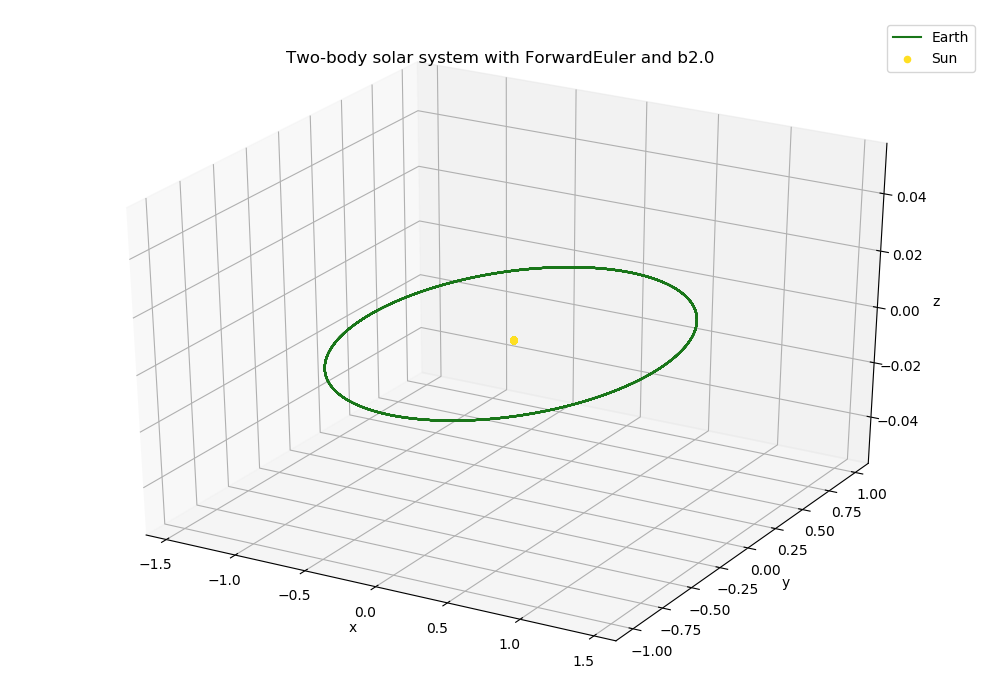
\includegraphics[width = 11cm]{img/plot3D_S_E_F_b20.png}
        \caption{CAPTIONHERE}
        \label{fig:plot3D_S_E_F_b20}
    \end{figure}

    \begin{figure}[H]
        \centering
        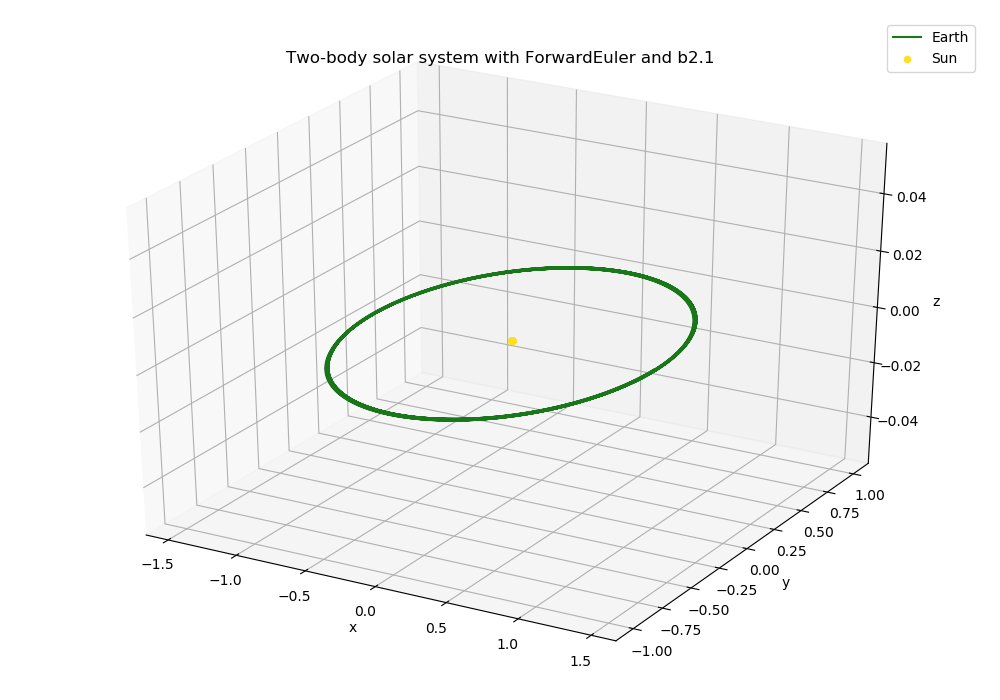
\includegraphics[width = 11cm]{img/plot3D_S_E_F_b21.png}
        \caption{CAPTIONHERE}
        \label{fig:plot3D_S_E_F_b21}
    \end{figure}

    \begin{figure}[H]
        \centering
        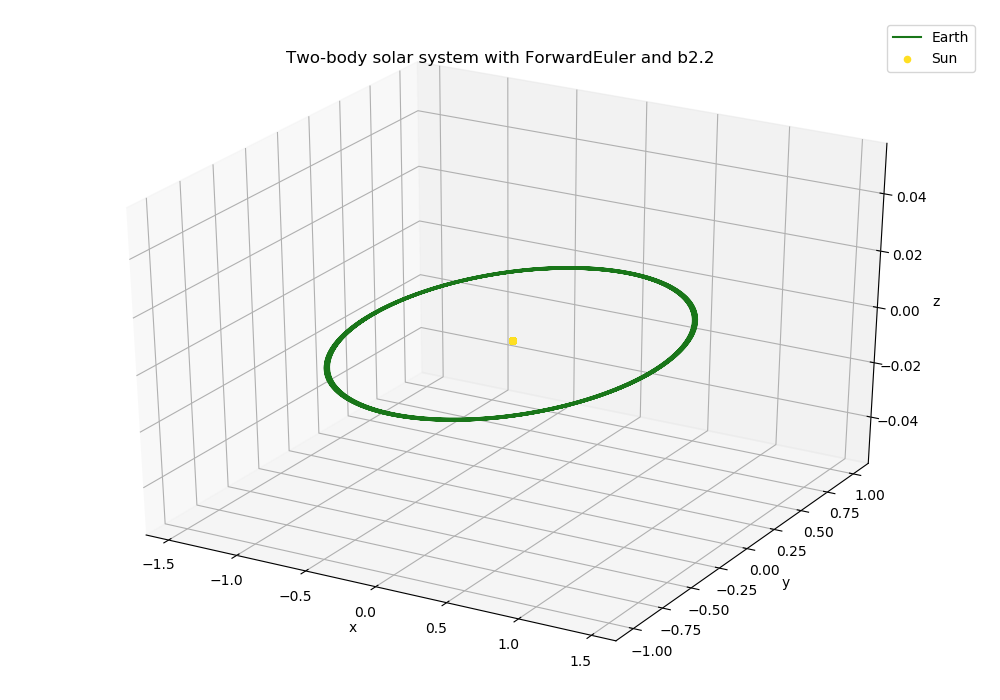
\includegraphics[width = 11cm]{img/plot3D_S_E_F_b22.png}
        \caption{CAPTIONHERE}
        \label{fig:plot3D_S_E_F_b22}
    \end{figure}

    \begin{figure}[H]
        \centering
        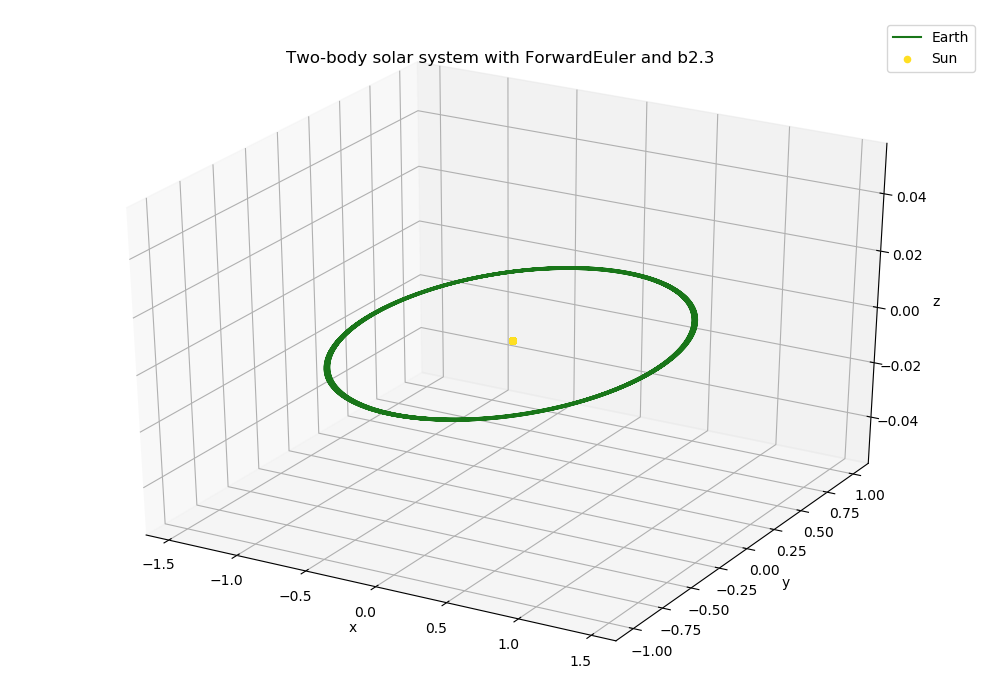
\includegraphics[width = 11cm]{img/plot3D_S_E_F_b23.png}
        \caption{CAPTIONHERE}
        \label{fig:plot3D_S_E_F_b23}
    \end{figure}

    \begin{figure}[H]
        \centering
        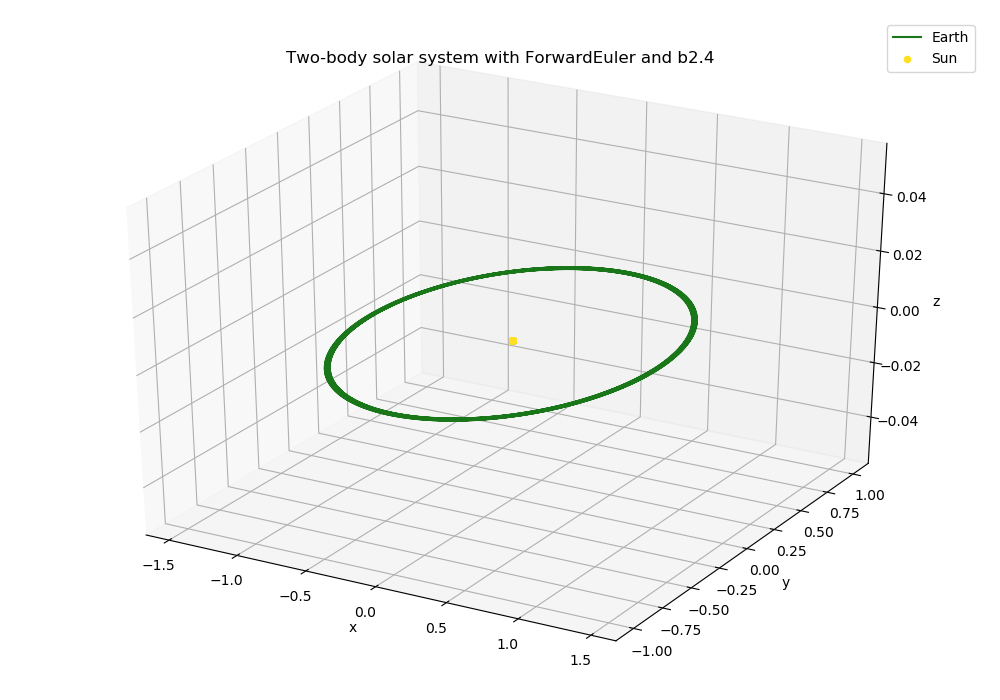
\includegraphics[width = 11cm]{img/plot3D_S_E_F_b24.png}
        \caption{CAPTIONHERE}
        \label{fig:plot3D_S_E_F_b24}
    \end{figure}

    \begin{figure}[H]
        \centering
        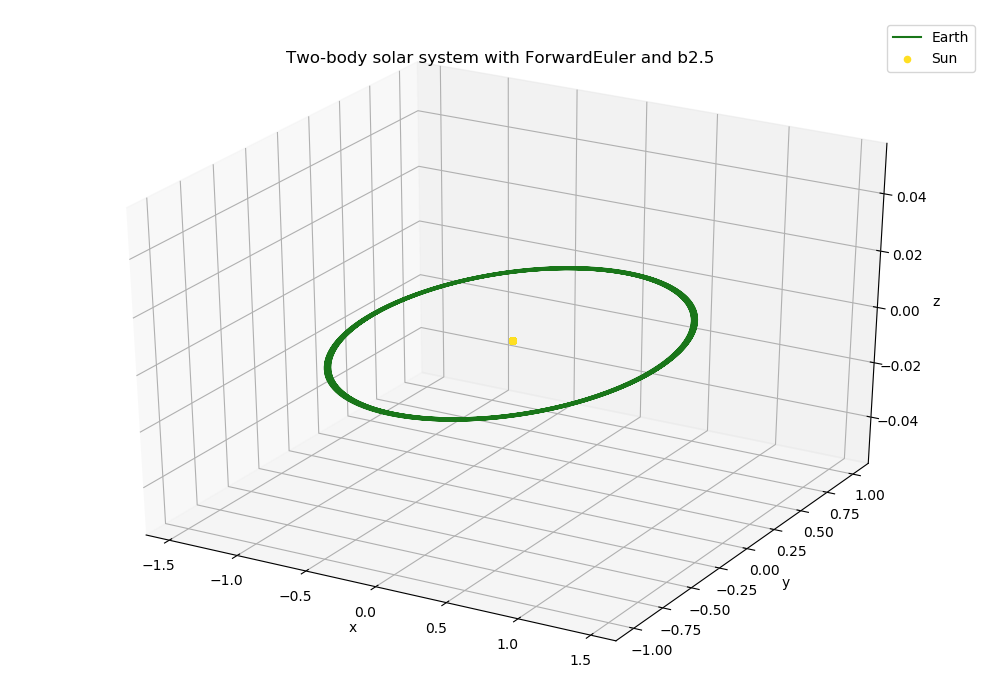
\includegraphics[width = 11cm]{img/plot3D_S_E_F_b25.png}
        \caption{CAPTIONHERE}
        \label{fig:plot3D_S_E_F_b25}
    \end{figure}

    \begin{figure}[H]
        \centering
        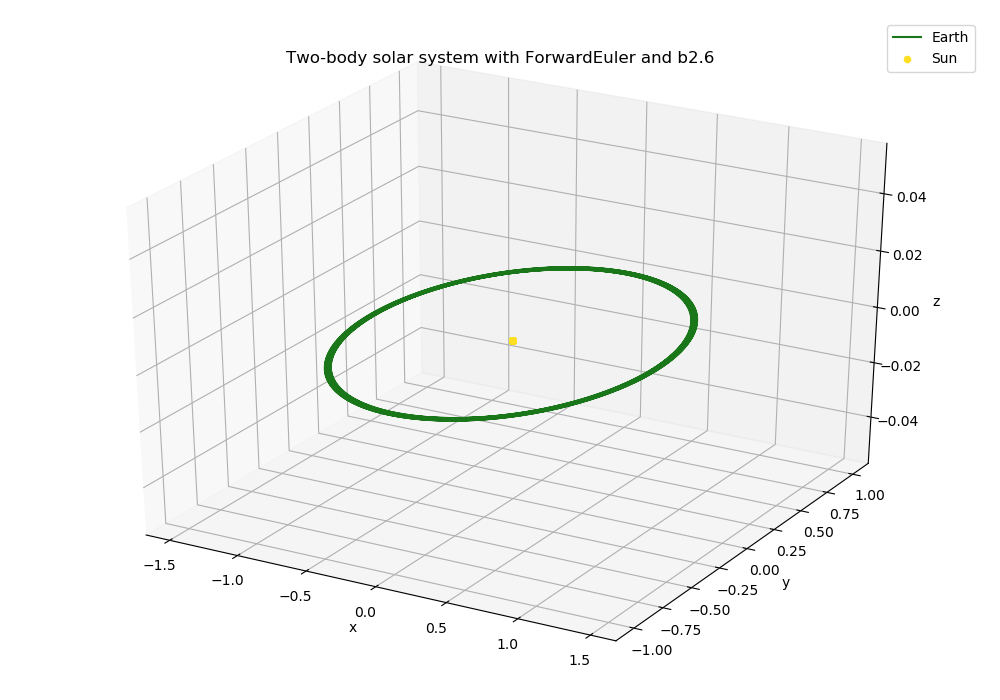
\includegraphics[width = 11cm]{img/plot3D_S_E_F_b26.png}
        \caption{CAPTIONHERE}
        \label{fig:plot3D_S_E_F_b26}
    \end{figure}

    \begin{figure}[H]
        \centering
        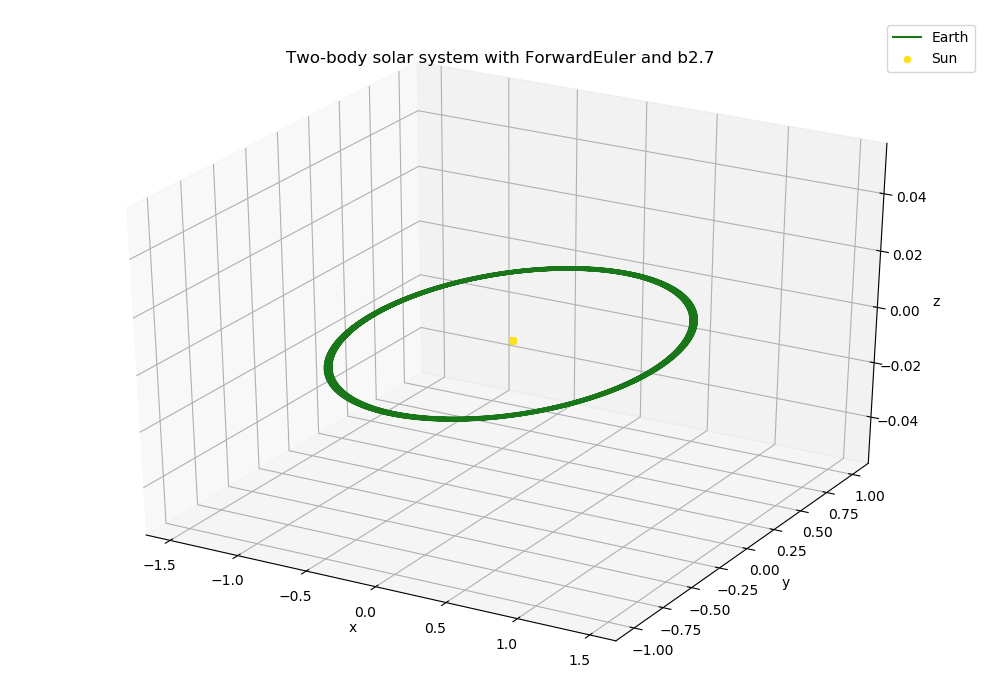
\includegraphics[width = 11cm]{img/plot3D_S_E_F_b27.png}
        \caption{CAPTIONHERE}
        \label{fig:plot3D_S_E_F_b27}
    \end{figure}

    \begin{figure}[H]
        \centering
        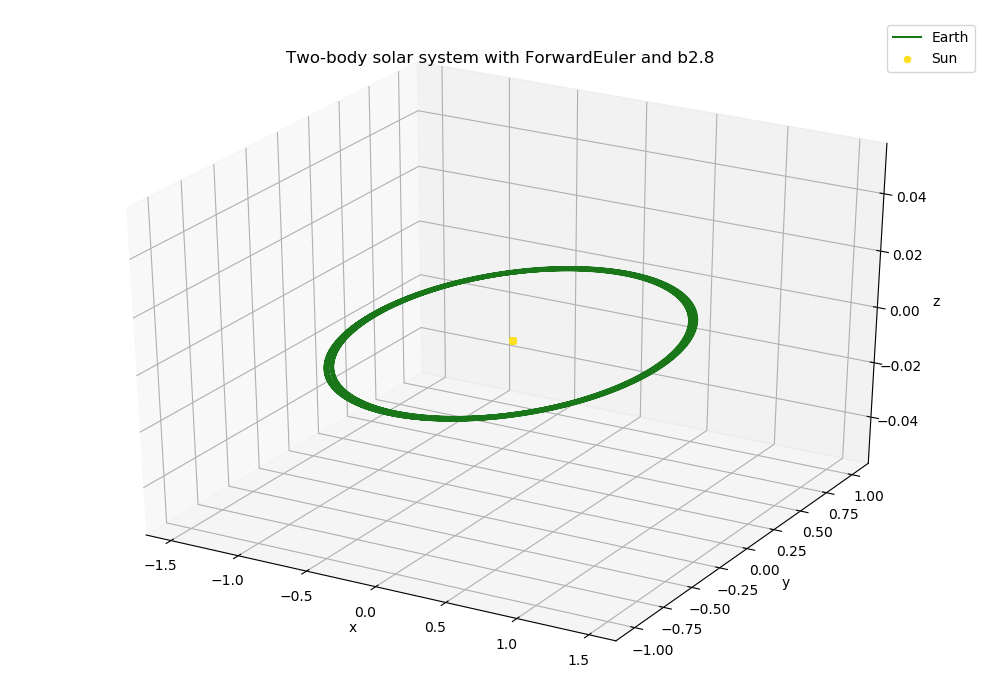
\includegraphics[width = 11cm]{img/plot3D_S_E_F_b28.png}
        \caption{CAPTIONHERE}
        \label{fig:plot3D_S_E_F_b28}
    \end{figure}

    \begin{figure}[H]
        \centering
        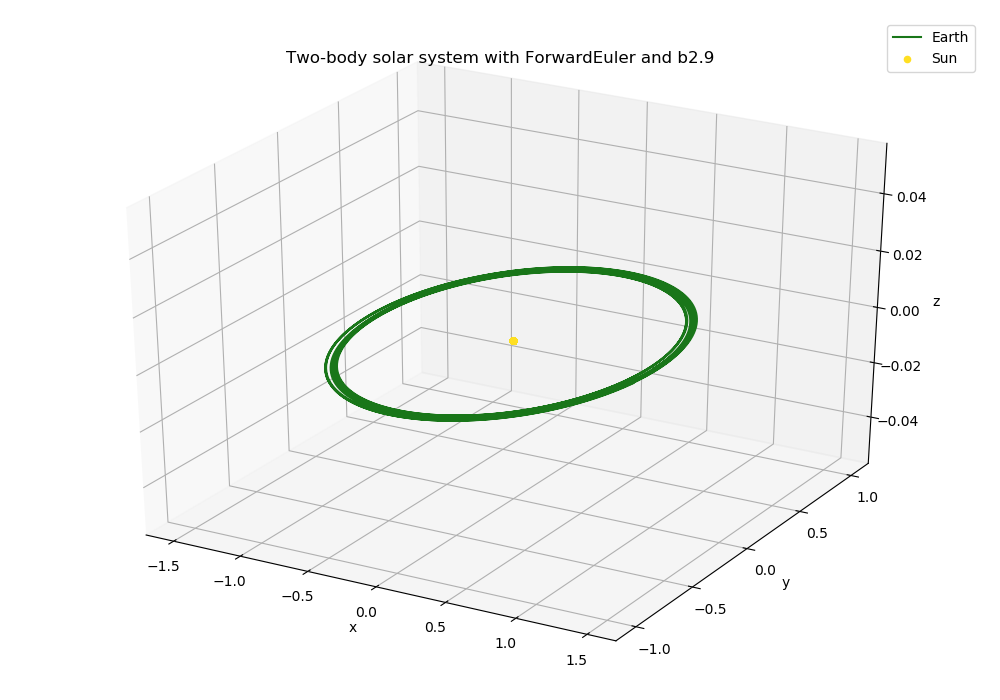
\includegraphics[width = 11cm]{img/plot3D_S_E_F_b29.png}
        \caption{CAPTIONHERE}
        \label{fig:plot3D_S_E_F_b29}
    \end{figure}

    \begin{figure}[H]
        \centering
        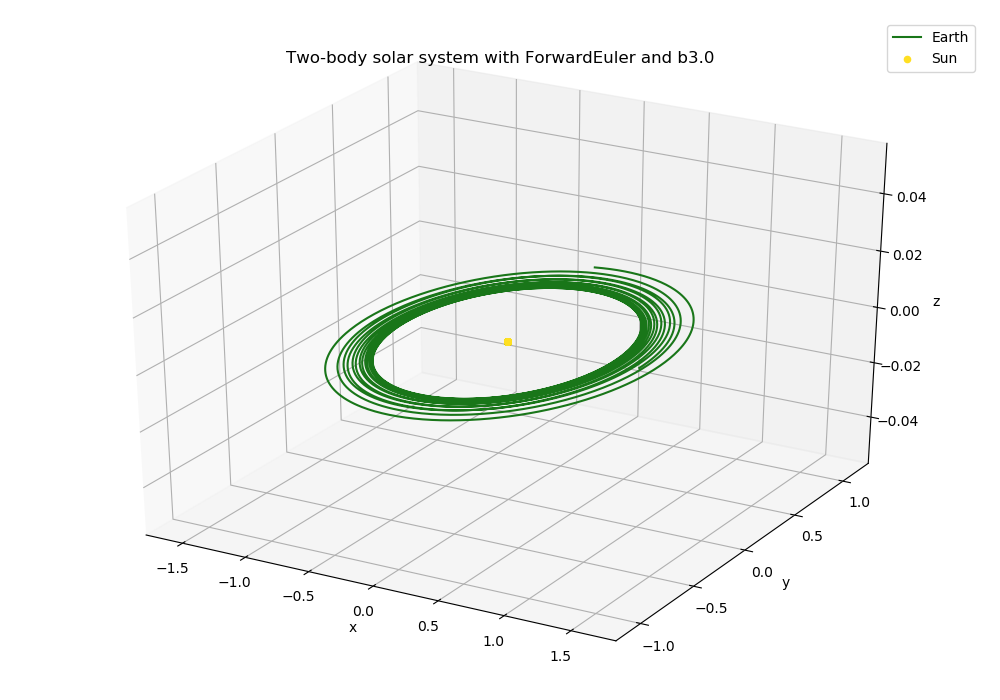
\includegraphics[width = 11cm]{img/plot3D_S_E_F_b30.png}
        \caption{CAPTIONHERE}
        \label{fig:plot3D_S_E_F_b30}
    \end{figure}

    \begin{figure}[H]
        \centering
        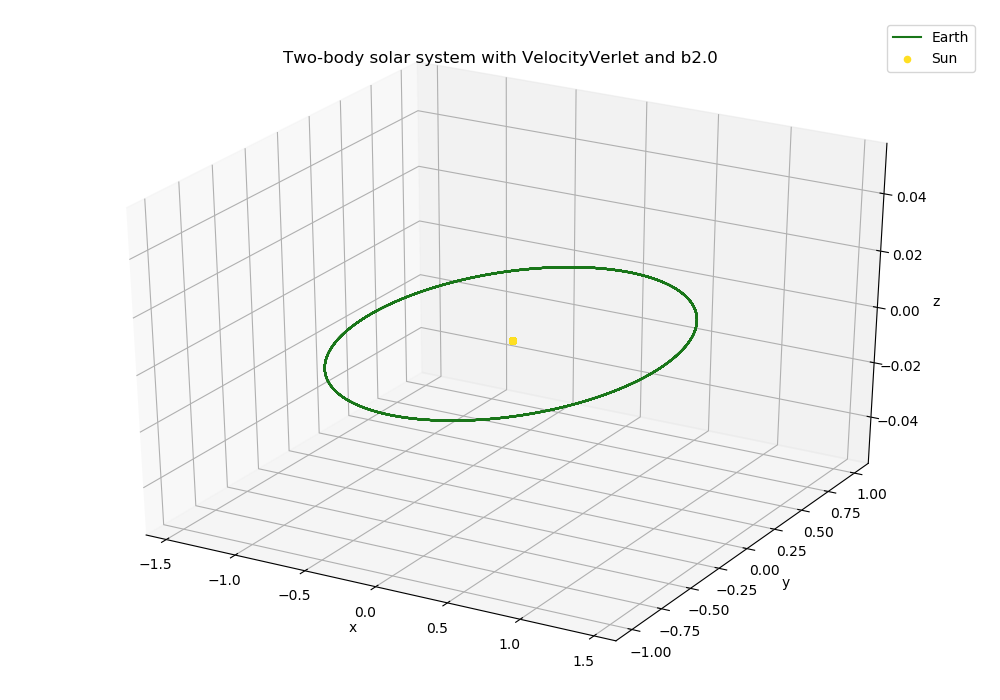
\includegraphics[width = 11cm]{img/plot3D_S_E_V_b20.png}
        \caption{CAPTIONHERE}
        \label{fig:plot3D_S_E_V_b20}
    \end{figure}

    \begin{figure}[H]
        \centering
        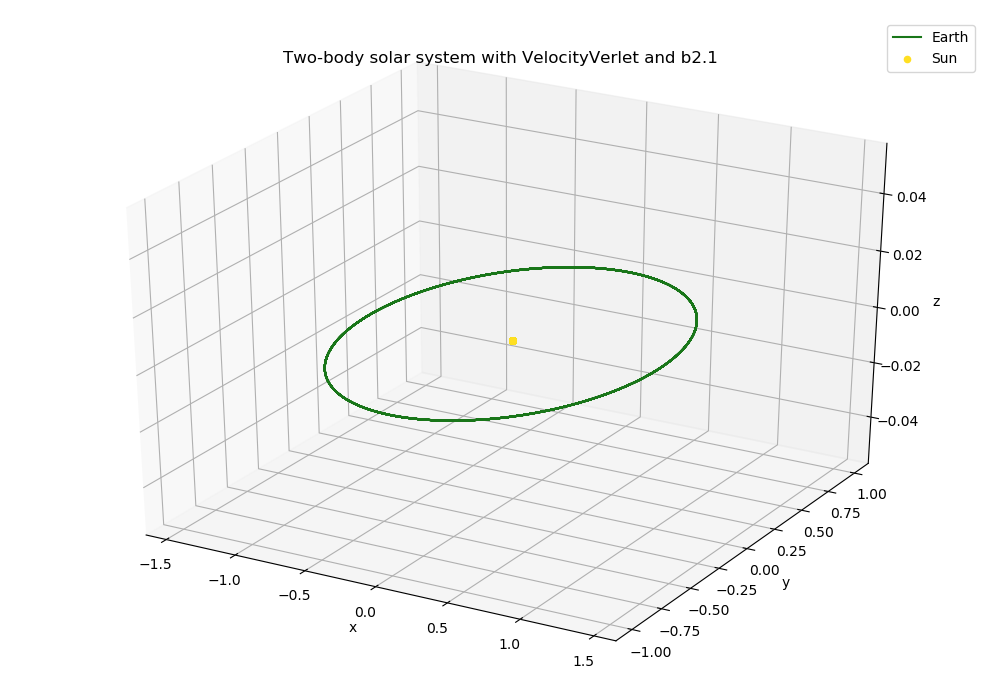
\includegraphics[width = 11cm]{img/plot3D_S_E_V_b21.png}
        \caption{CAPTIONHERE}
        \label{fig:plot3D_S_E_V_b21}
    \end{figure}

    \begin{figure}[H]
        \centering
        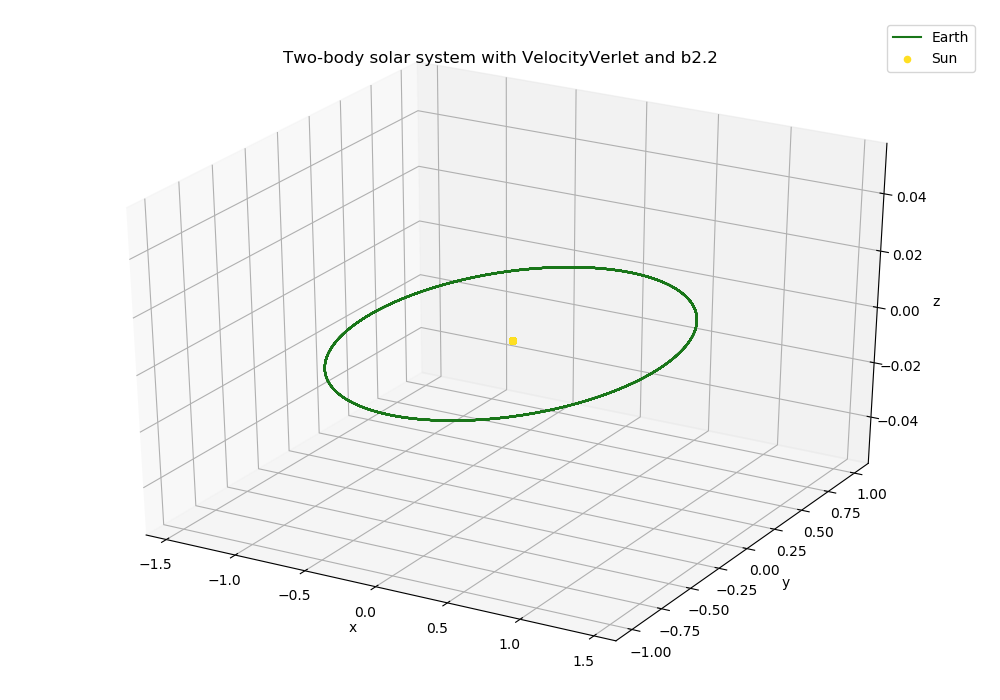
\includegraphics[width = 11cm]{img/plot3D_S_E_V_b22.png}
        \caption{CAPTIONHERE}
        \label{fig:plot3D_S_E_V_b22}
    \end{figure}

    \begin{figure}[H]
        \centering
        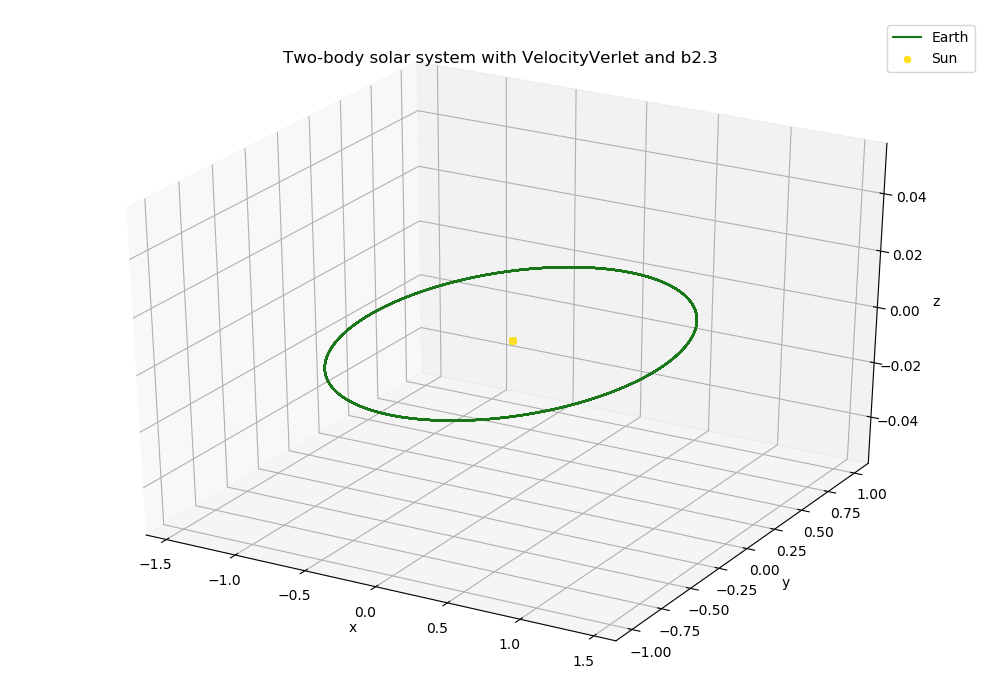
\includegraphics[width = 11cm]{img/plot3D_S_E_V_b23.png}
        \caption{CAPTIONHERE}
        \label{fig:plot3D_S_E_V_b23}
    \end{figure}

    \begin{figure}[H]
        \centering
        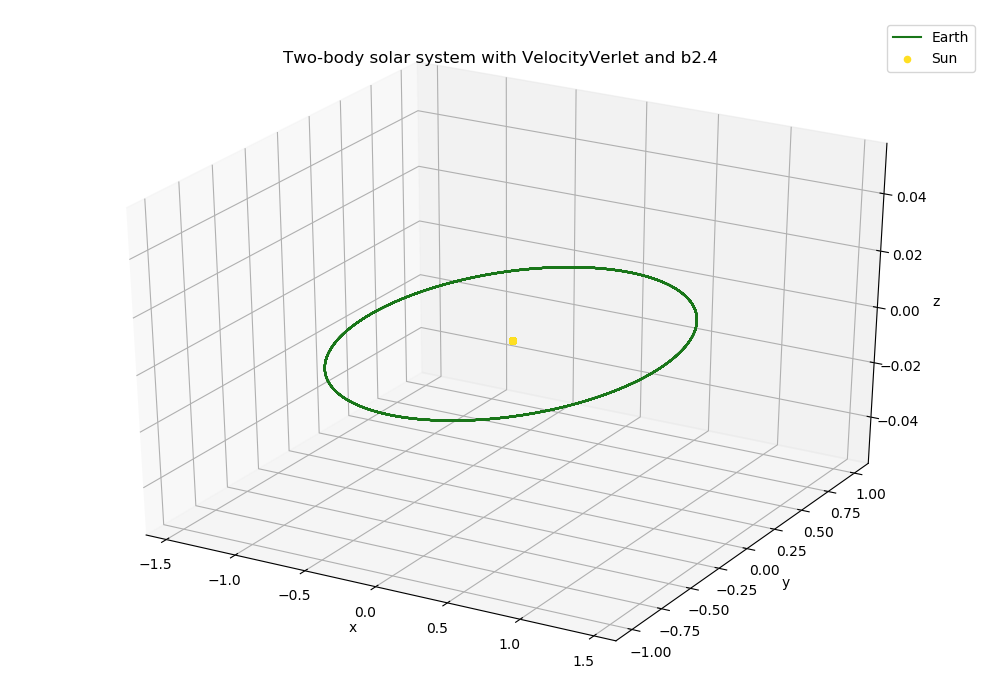
\includegraphics[width = 11cm]{img/plot3D_S_E_V_b24.png}
        \caption{CAPTIONHERE}
        \label{fig:plot3D_S_E_V_b24}
    \end{figure}

    \begin{figure}[H]
        \centering
        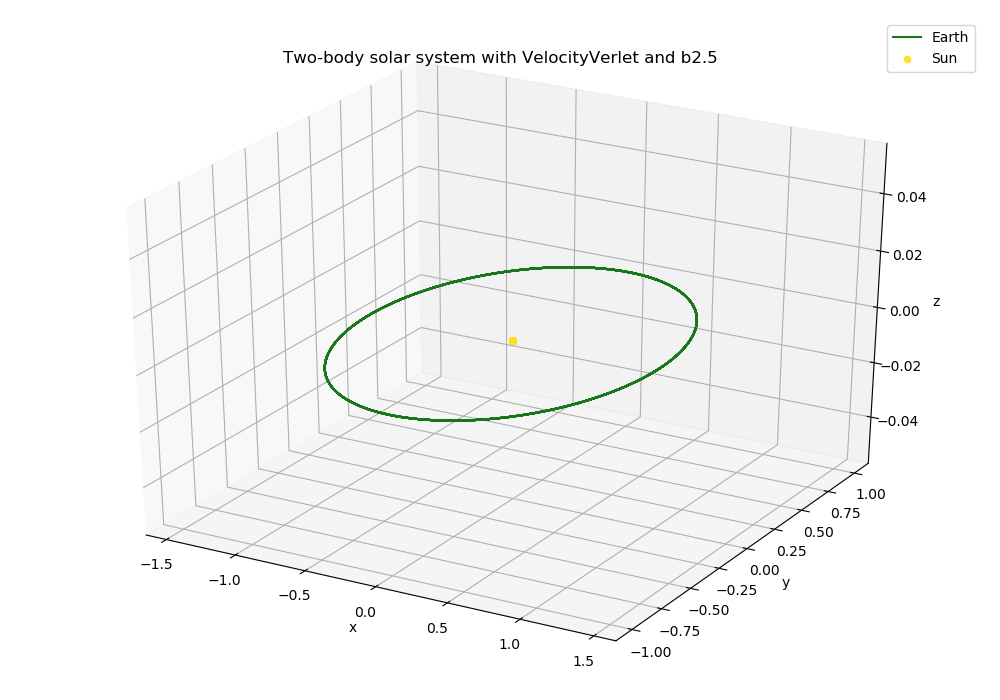
\includegraphics[width = 11cm]{img/plot3D_S_E_V_b25.png}
        \caption{CAPTIONHERE}
        \label{fig:plot3D_S_E_V_b25}
    \end{figure}

    \begin{figure}[H]
        \centering
        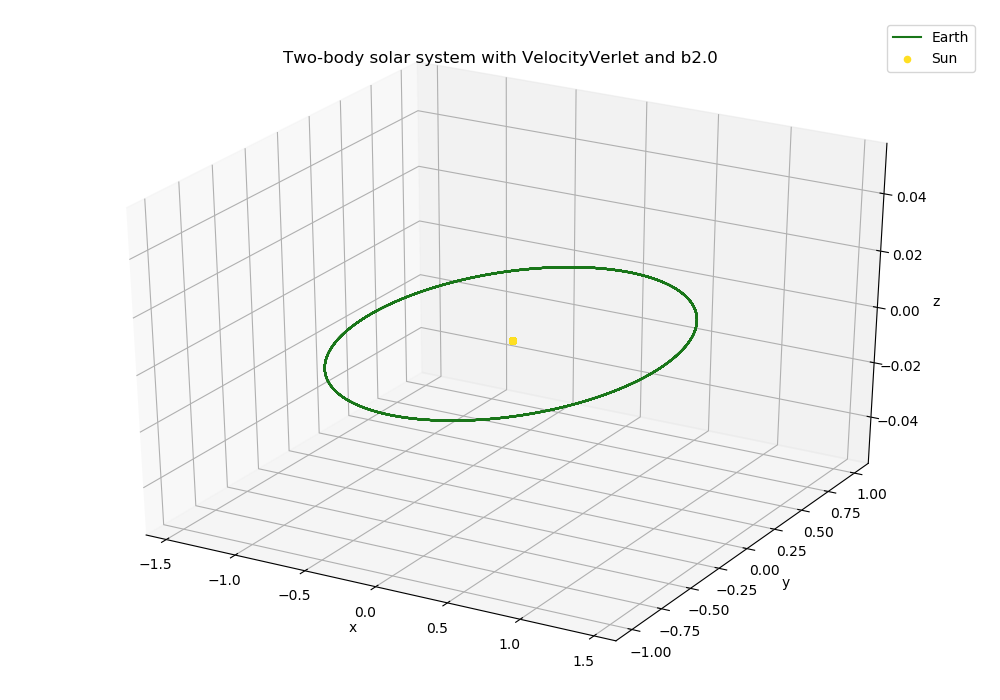
\includegraphics[width = 11cm]{img/plot3D_S_E_V_b20.png}
        \caption{CAPTIONHERE}
        \label{fig:plot3D_S_E_V_b26}
    \end{figure}

    \begin{figure}[H]
        \centering
        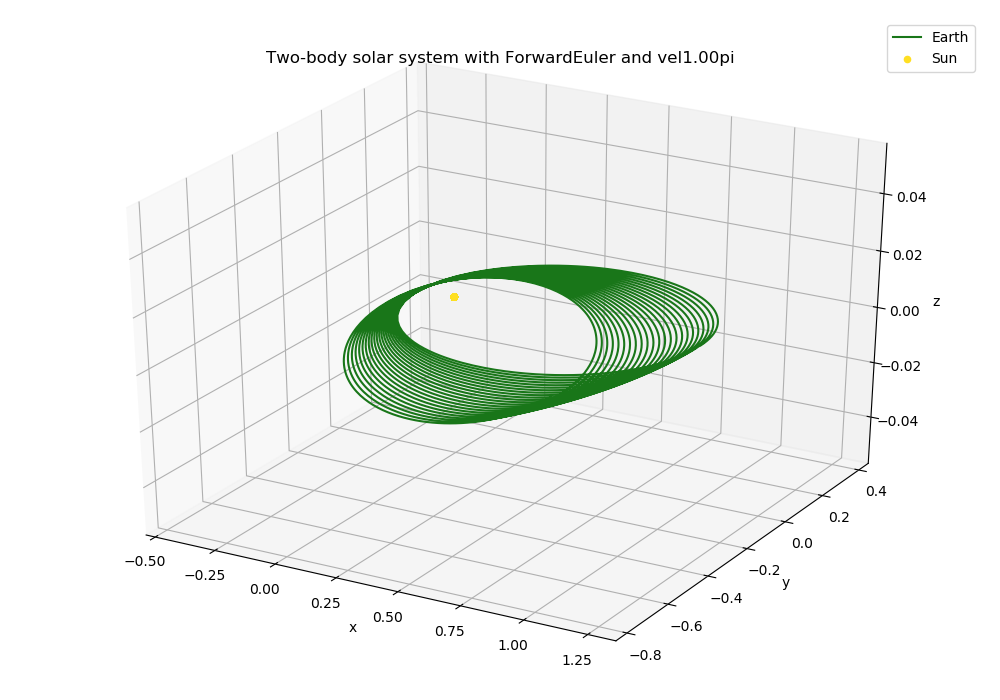
\includegraphics[width = 11cm]{img/plot3D_S_E_F_vel100pi.png}
        \caption{CAPTIONHERE}
        \label{fig:plot3D_S_E_F_vel100pi}
    \end{figure}

    \begin{figure}[H]
        \centering
        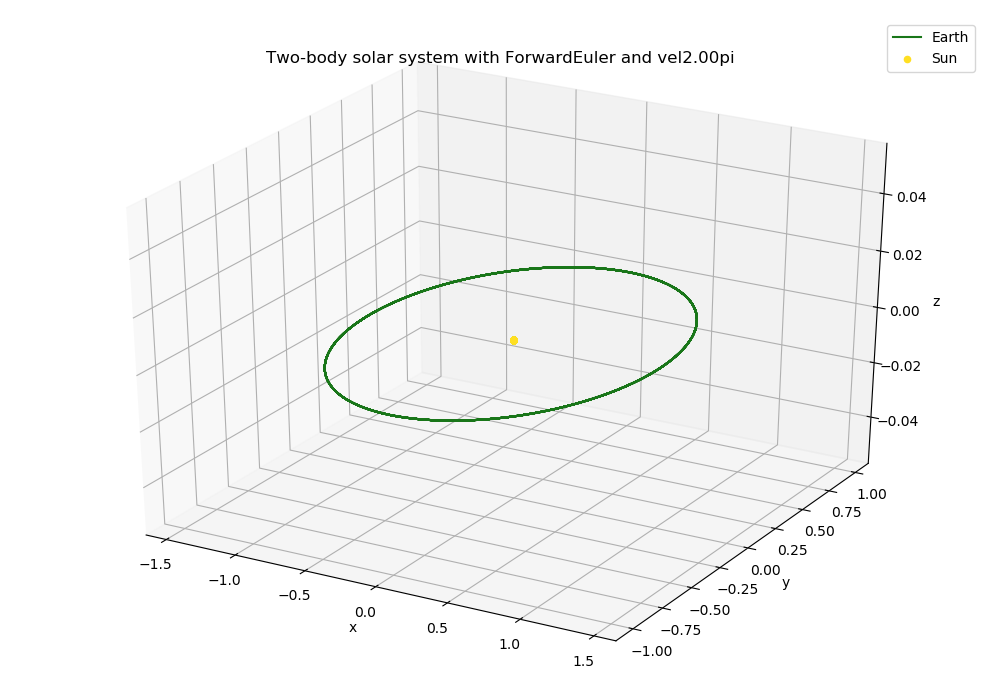
\includegraphics[width = 11cm]{img/plot3D_S_E_F_vel200pi.png}
        \caption{CAPTIONHERE}
        \label{fig:plot3D_S_E_F_vel200pi}
    \end{figure}

    \begin{figure}[H]
        \centering
        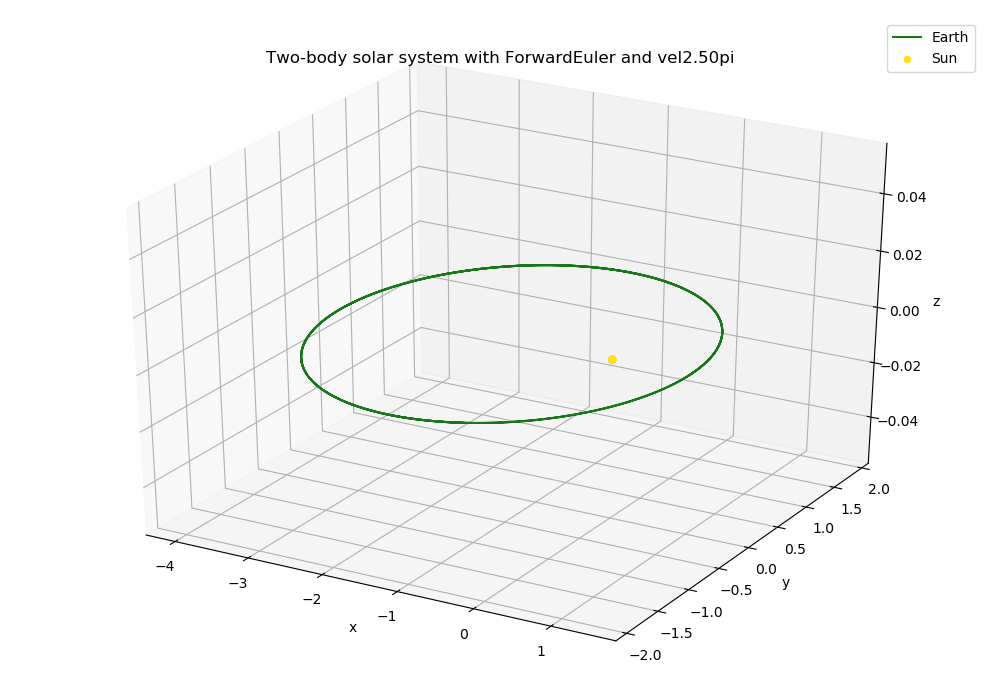
\includegraphics[width = 11cm]{img/plot3D_S_E_F_vel250pi.png}
        \caption{CAPTIONHERE}
        \label{fig:plot3D_S_E_F_vel250pi}
    \end{figure}

    \begin{figure}[H]
        \centering
        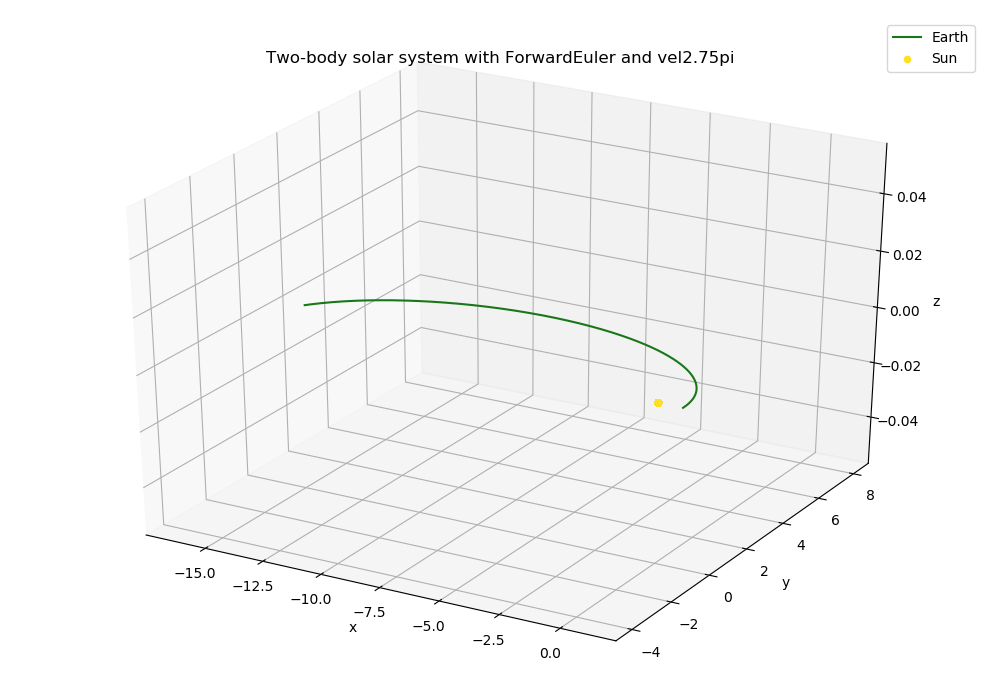
\includegraphics[width = 11cm]{img/plot3D_S_E_F_vel275pi.png}
        \caption{CAPTIONHERE}
        \label{fig:plot3D_S_E_F_vel275pi}
    \end{figure}

    \begin{figure}[H]
        \centering
        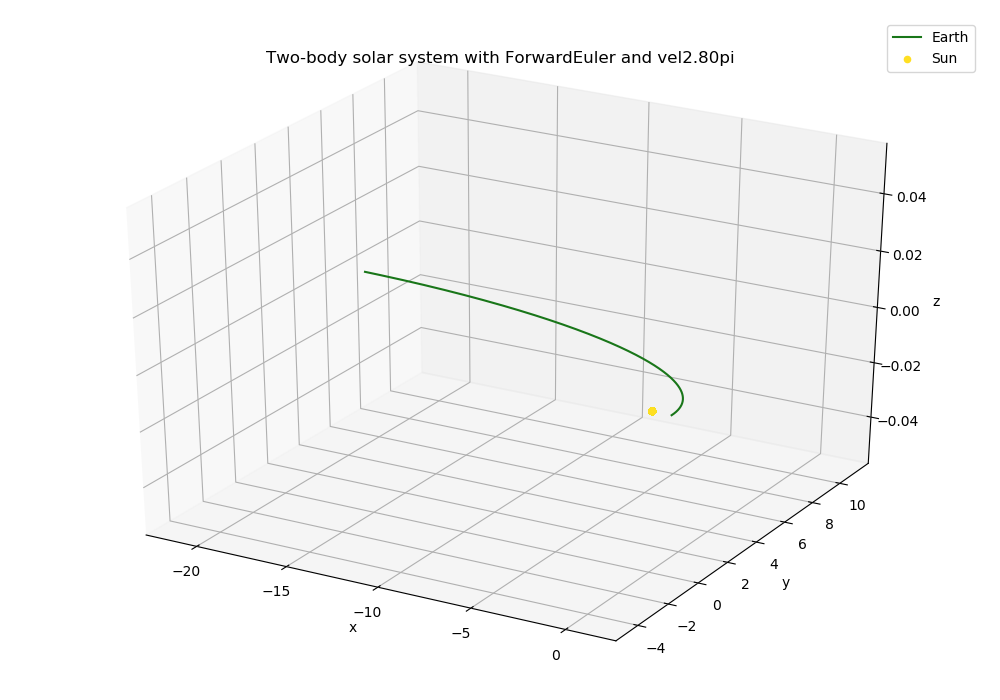
\includegraphics[width = 11cm]{img/plot3D_S_E_F_vel280pi.png}
        \caption{CAPTIONHERE}
        \label{fig:plot3D_S_E_F_vel280pi}
    \end{figure}

    \begin{figure}[H]
        \centering
        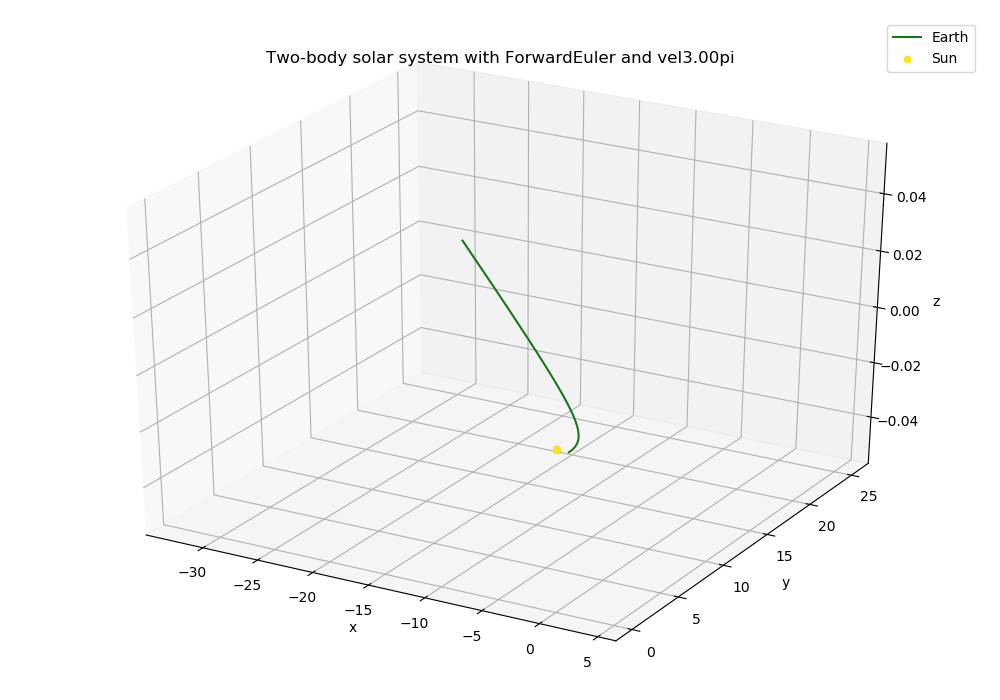
\includegraphics[width = 11cm]{img/plot3D_S_E_F_vel300pi.png}
        \caption{CAPTIONHERE}
        \label{fig:plot3D_S_E_F_vel300pi}
    \end{figure}

    \begin{figure}[H]
        \centering
        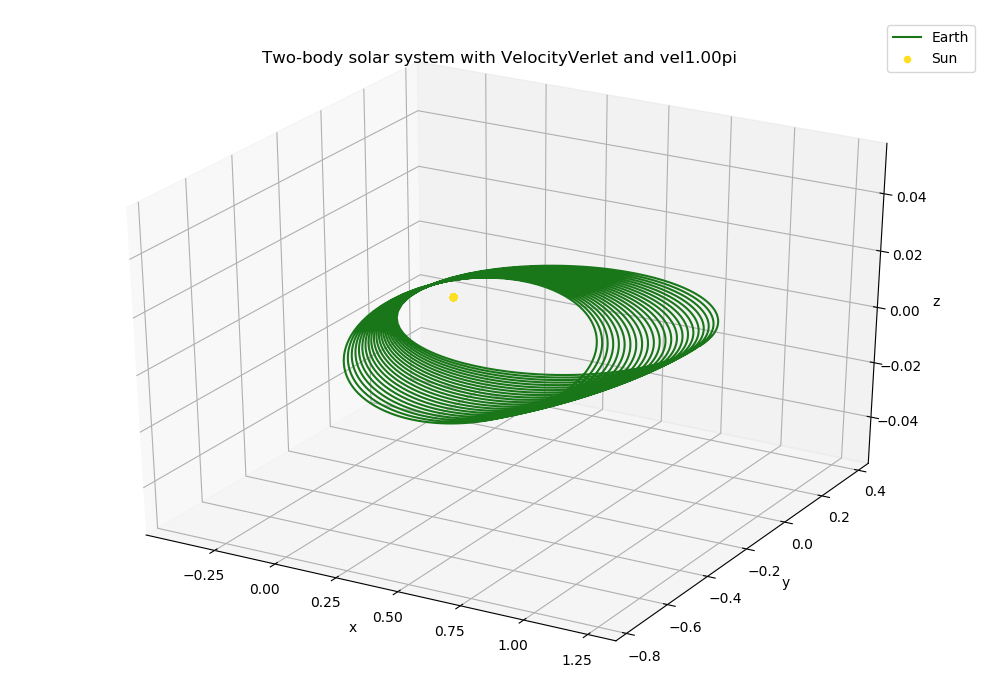
\includegraphics[width = 11cm]{img/plot3D_S_E_V_vel100pi.png}
        \caption{CAPTIONHERE}
        \label{fig:plot3D_S_E_V_vel100pi}
    \end{figure}

    \begin{figure}[H]
        \centering
        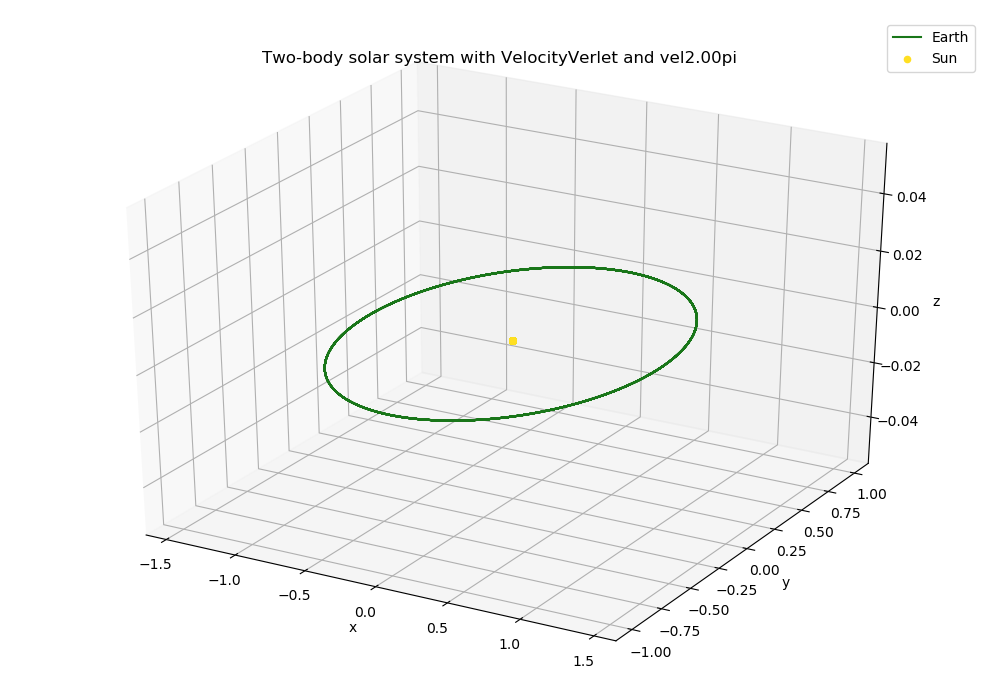
\includegraphics[width = 11cm]{img/plot3D_S_E_V_vel200pi.png}
        \caption{CAPTIONHERE}
        \label{fig:plot3D_S_E_V_vel200pi}
    \end{figure}

    \begin{figure}[H]
        \centering
        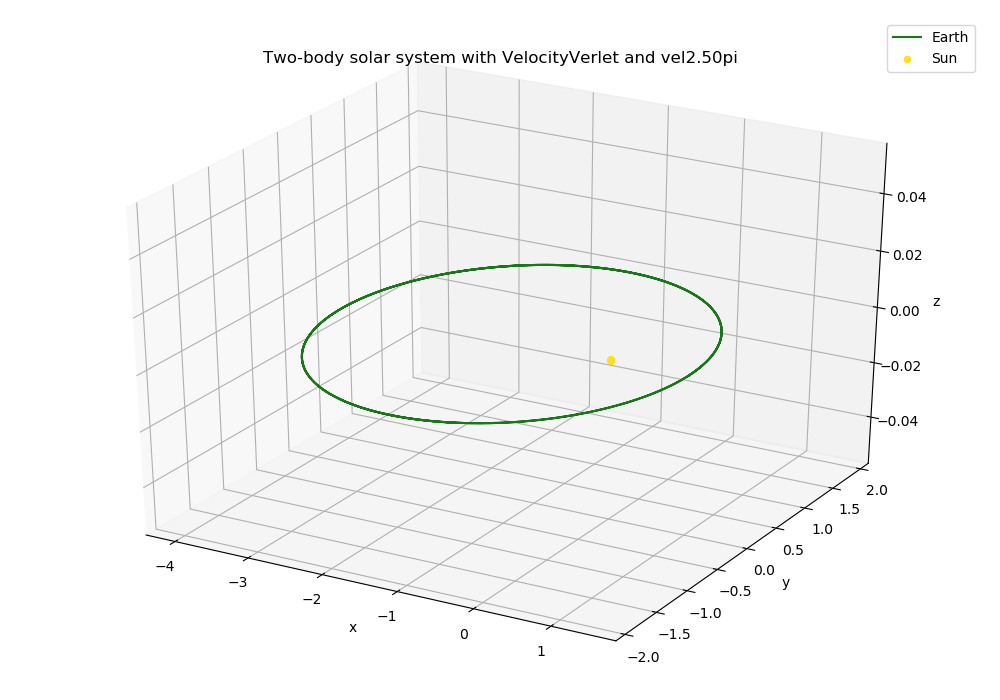
\includegraphics[width = 11cm]{img/plot3D_S_E_V_vel250pi.png}
        \caption{CAPTIONHERE}
        \label{fig:plot3D_S_E_V_vel250pi}
    \end{figure}

    \begin{figure}[H]
        \centering
        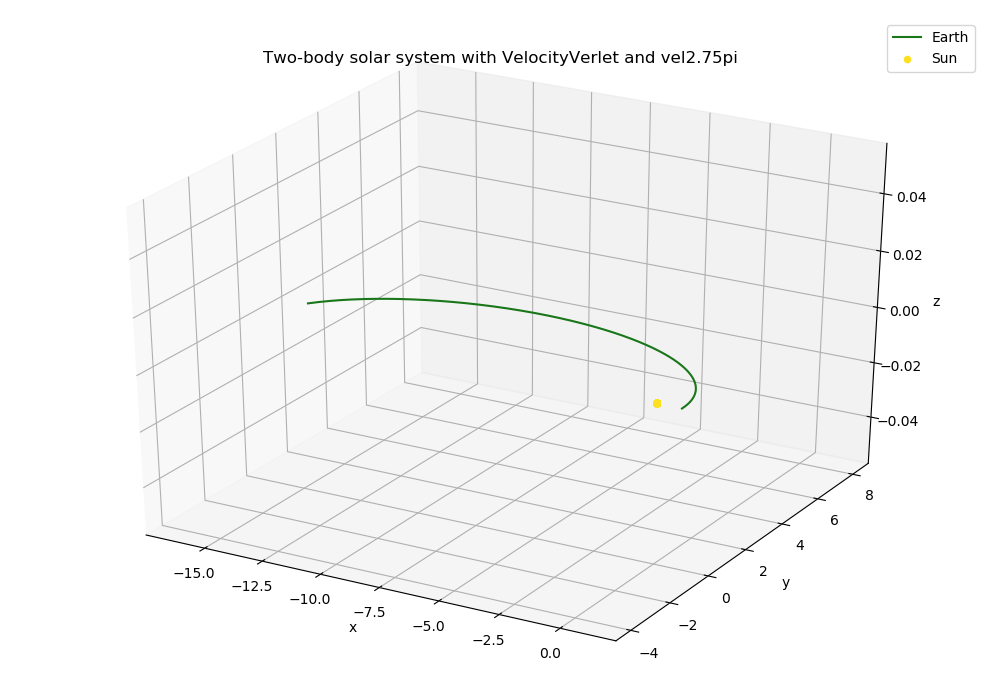
\includegraphics[width = 11cm]{img/plot3D_S_E_V_vel275pi.png}
        \caption{CAPTIONHERE}
        \label{fig:plot3D_S_E_V_vel275pi}
    \end{figure}

    \begin{figure}[H]
        \centering
        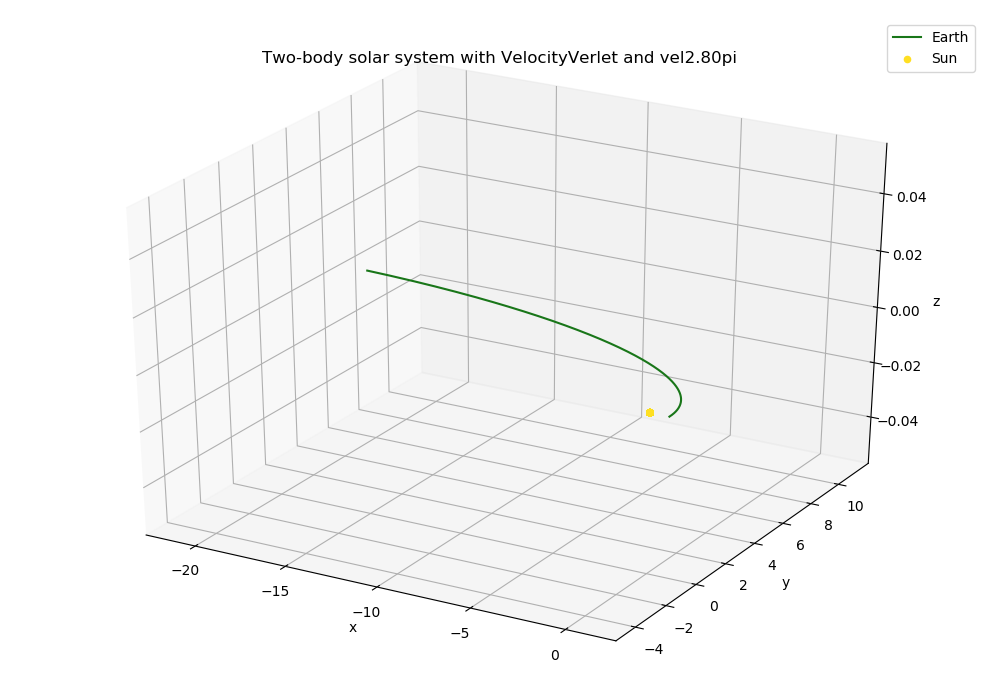
\includegraphics[width = 11cm]{img/plot3D_S_E_V_vel280pi.png}
        \caption{CAPTIONHERE}
        \label{fig:plot3D_S_E_V_vel280pi}
    \end{figure}

    \begin{figure}[H]
        \centering
        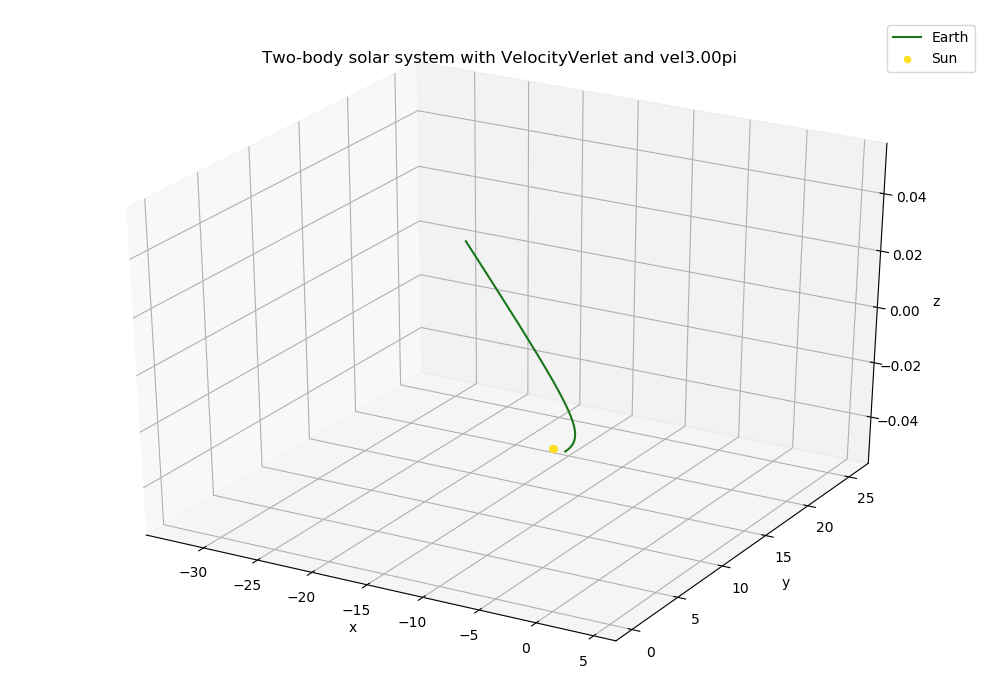
\includegraphics[width = 11cm]{img/plot3D_S_E_V_vel300pi.png}
        \caption{CAPTIONHERE}
        \label{fig:plot3D_S_E_V_vel300pi}
    \end{figure}


\iffalse
    \begin{table}[H]
      \centering
      \caption{CAPTION HERE}
      \vspace{2mm}
      \label{tab:LABELHERE}
      \begin{tabular}{|c|c|}
          \hline
           x & y\\
          \hline \hline
          x1 & y1 \\
          x2 & y2 \\
          x3 & y3 \\
          x4 & y4 \\
          x5 & y5 \\
          \hline
      \end{tabular} \\
      \hspace{0pt}\\
    \end{table}
\fi

%--------------- Discussion ---------------------------------------
\vspace{1cm}

\clearpage
\newpage

\section{Discussion} \label{sec:Discussion}

 and discussion


 Give a critical discussion of your work and place it in the correct context.
 Relate your work to other calculations/studies

%---------------Conclusion and perspective---------------------------
\vspace{1cm}

\section{Conclusion and perspective} \label{sec:Conclusion}

Conclusions and perspectives


What should I focus on? Conclusions.
State your main findings and interpretations
Try as far as possible to present perspectives for future work
Try to discuss the pros and cons of the methods and possible improvements

%----------------References----------------------------------------

\vspace{1cm}

\section{References} \label{sec:References}

\iffalse
What should I focus on? References.
Give always references to material you base your work on, either scientific articles/reports or books.
Refer to articles as: name(s) of author(s), journal, volume (boldfaced), page and year in parenthesis.
Refer to books as: name(s) of author(s), title of book, publisher, place and year, eventual page numbers
\fi

\begin{thebibliography}{}

\bibitem{task}
Morten H. Jensen (2019), \href{https://github.com/CompPhysics/ComputationalPhysics/blob/master/doc/Projects/2019/Project5/SolarSystem/pdf/SolarSystem.pdf}{Project 5}, Departement of Physics, University of Oslo, Norway

\bibitem{github}
Erik B. Grammeltvedt, Alexandra Jahr Kolstad, Erlend T. North (2019), \href{https://github.com/Erikbgram/Fys3150}{GitHub}, Students of Departement of Physics, University of Oslo, Norway

\bibitem{lecture_slides}
Morten H. Jensen (2015), \href{https://github.com/CompPhysics/ComputationalPhysics/blob/master/doc/Lectures/lectures2015.pdf}{Lecture slides for FYS3150}, Department of Physics, University of Oslo, Norway

\bibitem{solarsystemdata}
Jon. D. Giorgini (2019), \href{https://ssd.jpl.nasa.gov/horizons.cgi#top}{Physical data of the planets and the sun.}, Solar System Dynamics Group, Horizons On-Line Ephemeris System, Jet Propulsion Laboratory, Pasadena, California, USA


\end{thebibliography}


%--------------Appendix---------------------------------------------
\vspace{1cm}


\appendix
\section{Appendix} \label{sec:Appendix}

Appendix with extra material


What should I focus on? additional material.
Additional calculations used to validate the codes
Selected calculations, these can be listed with few comments
Listing of the code if you feel this is necessary
You can consider moving parts of the material from the methods section to the appendix. You can also place additional material on your webpage.

\subsection{Mass-conversion} \label{app:mass}


    \begin{table}[H]
        \centering
        \caption{Astronomical data retrieved from \cite{solarsystemdata}. }
        \vspace{2mm}
        \label{tab:mass}
        \begin{tabular}{|c|c|c|c|}
            \hline
            Celestial Body & Mass [kg] & Mass [$M_{\odot}$] & Distance to sun [AU]\\
            \hline \hline
            Sun     & $ 2    \cdot10^{30} $ & 1                    & 0 \\
            Mercury & $ 3.3  \cdot10^{23} $ & $1.65 \cdot 10^{-7}$ & 0.39 \\
            Venus   & $ 4.9  \cdot10^{24} $ & $2.45 \cdot 10^{-6}$ & 0.72 \\
            Earth   & $ 6    \cdot10^{24} $ & $3.0 \cdot 10^{-6}$  & 1 \\
            Mars    & $ 6.6  \cdot10^{23} $ & $3.3 \cdot 10^{-7}$  & 1.52 \\
            Jupiter & $ 1.9  \cdot10^{27} $ & $9.5 \cdot 10^{-4}$  & 5.20 \\
            Saturn  & $ 5.5  \cdot10^{26} $ & $2.75 \cdot 10^{-4}$ & 9.54 \\
            Uranus  & $ 8.8  \cdot10^{25} $ & $4.4 \cdot 10^{-5}$  & 19.19 \\
            Neptune & $ 1.03 \cdot10^{26} $ & $5.15 \cdot 10^{-5}$ & 30.06 \\
            Pluto   & $ 1.31 \cdot10^{22} $ & $6.55 \cdot 10^{-9}$ & 39.53 \\
            \hline
        \end{tabular} \\
        \hspace{0pt}\\
    \end{table}

\subsection{Explaining the calculation of a planets escape velocity} \label{sec:escapevelocity}

    As some of these problems are soluble by hand there are some calculations that can be done prior to the simulations in order to have something to compere results with. For instance one can quite easily calculate a planets escape velocity from the sun. One can use that that the escape velocity would be the lowest energy required to move the planet out of the gravitational pool from the sun. In that case the planet would be left with zero kinetic energy. Because the planet is moved out of the gravitational field the potential energy would also bee 0. Therefore the expression for the system will be given as. This is with the condition that there is no other forces acting on the system except for the gravitational force.   \\

    $U_i + K_i = U_f + K_f$ \\

    Due too the criteria we have sett for the model and the need for conservation of energy the expretion becomes: \\

    $U_i + K_i = 0 + 0$ \\

    The potential energy is given by, the gravitational potential which is:\\

    $P = - \frac{GMm}{r}$ \\

    The kinetic energy is given by the planets kinetic energy: \\

    $k = \frac{1}{2} mv_p$ \\

    Therefore the escape velocity can be calculated as the kinetic energy being equal to the potential energy. \\

    \begin{equation} \label{eq:escapevelocity}
        v_p =  \sqrt{\frac{2GM}{r}}
    \end{equation}


\subsection{Rewriting Newtons second law of motion} \label{sec:n2l}

    Newtons second law of motion is stated in equation (1).

    \begin{equation} \label{eq:n2l}
        F = ma  (1)\\
    \end{equation}


    Equation (1) can be written as a differential equation that will give the force as a function of position (2).\\

    \begin{equation}    \label{eq:diffn2l}
        F(x,t) = m\frac{d^{2}x}{dt^{2}} (2)\\
    \end{equation}

    Since we know that the velocity,v, is given as a function of change in position over change in time. This gies us equation (3).\\

    \begin{equation}    \label{eq:diffvelocity}
        v(x,t) = \frac{dx}{dt} (3) \\
    \end{equation}

    Using equation (1),(2) and (3), one can now created two coupled differential equations. The first one is (3) and the second one is (4). (4) is a combination of (1) , (2) and (3). \\

    \begin{equation}    \label{eq:acceleration}
        \frac{dv}{dt} = F(x,t)/m = a(x,t) (4) \\
    \end{equation}

    Solving this system fro x with a tailor expantion one gets (5).\\

    \begin{equation}    \label{eq:positiontaylor}
        x(t+h) = x(t) + hx^{1}(t) + \frac{h^{2}}{2} x^{2}(t) + Oh^{4} (5)\\
    \end{equation}

    From equation (3) and (4) we have that $a(x,t) = x^{2}(t)$. Using equation (3), $x^{1}(t) = v(x,t)$ This can now be substituted in too equation (5). And gives equation (6).  \\

    \begin{equation}    \label{eq:positionfinal}
        x(t+h) = x(t) + h v(x,t) + \frac{h^{2}}{2} a(x,t) + (O)h^{4} (6) \\
    \end{equation}

    As one can see from the equation the system has a troncation error of $(O)h^{4}$.
    Using a Tayler expansion for the velocity as well as for the position. \\

    \begin{equation}    \label{eq:velocityfinal}
        v(t+h) = v(t) + h v^{1}(x,t) + \frac{h^{2}}{2}v(t) (7) \\
    \end{equation}

    It is important to discretize the expressions as they are the ones that will be used in the program. This changes x(t+h) too x(i+1). \\



\subsection{Adjusting Newtons method for relativity}






%----------------Slutten av dokumentet---------------------------------------


%\end{multicols}

\end{document}
